\section{Motion Processor Unit}
An accelerometer will be needed to detect when a distress call should be signaled. Figure \ref{accel} shows the Sparkfun IMU Breakout MPU-9250 that will be used throughout this project, which features a 3-axis accelerometer. When an object of specific weight falls into the water, it causes water ripples of certain magnitude to spread throughout the water. A change in acceleration of the waves then causes an applied force on the MPU. This force causes a disturbance in capacitance between micro-structures within the MPU that is identified through internal circuitry \cite{acceler}. Another feature of the Sparkfun MPU an inetgrated 3-axis gyroscope. The gyroscope can be helpful by identifying a specific change in angular velocity. By configuring the MPU onto a Raspberry-Pi microcontroller, an effective motion detection device can be achieved. \hfill
\newline

\begin{figure}[H]
\centering
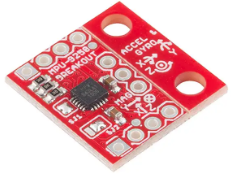
\includegraphics[width = 6.5cm,height = 4.5cm]{graphics/Accelerometer.PNG}

\caption{Sparkfun IMU Breakout MPU-9250 Board}
\label{accel}
 
\end{figure}